\chapter{Date de antrenament}
\section{Colectarea și salvarea datelor}
Datele de antrenament sunt extrem de importante.
O expresie populară\footnote{Expresia este ``garbage in, garbage out'', iar o expresie românească similară ar fi ``semeni vânt, culegi furtună''} ne spune că dacă datele furnizate algorimilor de învățare automată sunt de proastă calitate, atunci așa va fi și performanța acelor algoritmi, sau mai bine spus a modelelor matematice și a generalizărilor create de aceștia.
Mulțimea de date trebuie să conțină varietate, în cazul de față însemnând poze cu fundaluri diferite, condiții de iluminare diverse ș.a.m.d.

Am lucrat cu imagini cu utilizatorul, capturate prin webcam.
Apoi, am extras fie doar fața acestuia din imagine, fie doar un ochi, fie o porțiune dreptunghiulară în care se regăsesc ambii ochi.
Pentru fiecare experiment realizat, am menționat ce date au fost folosite și în ce mod au fost procesate acestea.

\begin{lstlisting}[language=Python, caption=Colectarea datelor]
def start_collecting(self, collection_type):
    dc_logger.info(f'Start collecting data in {collection_type} mode')
    WebcamCapturer.start_capturing()
    self.gui.start()
    dc_logger.info('DataCollectorGUI started')
    if collection_type == 'background':
        self.mouse_listener.start_listening()
        dc_logger.info('Mouse listener started')
    elif collection_type == 'active':
        threading.Thread(target=self.start_active_collection).start()
\end{lstlisting}

Când colectarea datelor este gata, acestea sunt salvate sub forma unei ``sesiuni''.
Fiecare sesiune este definită de numărul imaginilor care au fost capturate, de rezoluția ecranului și rezoluția webcam-ului.
Mai jos se poate observa structura directoarelor și modul în care aceste date sunt salvate, fără a aplica vreo modificare.

\begin{lstlisting}[language=Python, caption=Salvarea datelor]
def save_collected_data(self):
    if len(self.collected_data) == 0:
        return
    dc_logger.info(
        f'Acquiring lock for data collection. Locked = {self.collect_data_lock.locked()}')
    self.collect_data_lock.acquire()
    dc_logger.info('Lock acquired')
    session_no = self.get_session_number()
    dc_logger.info(f"Saving data for session_{session_no}")
    self.save_session_info(session_no)
    self.save_images_info(session_no)
    self.save_images(session_no)
    self.collect_data_lock.release()
    self.collected_data = []
    dc_logger.info('Saving data done')
\end{lstlisting}


\begin{figure}[ht]
    \centering
    
\includegraphics[width=0.49\textwidth]{data_structure_1.png}
    
\includegraphics[width=0.49\textwidth]{data_structure_2.png}
    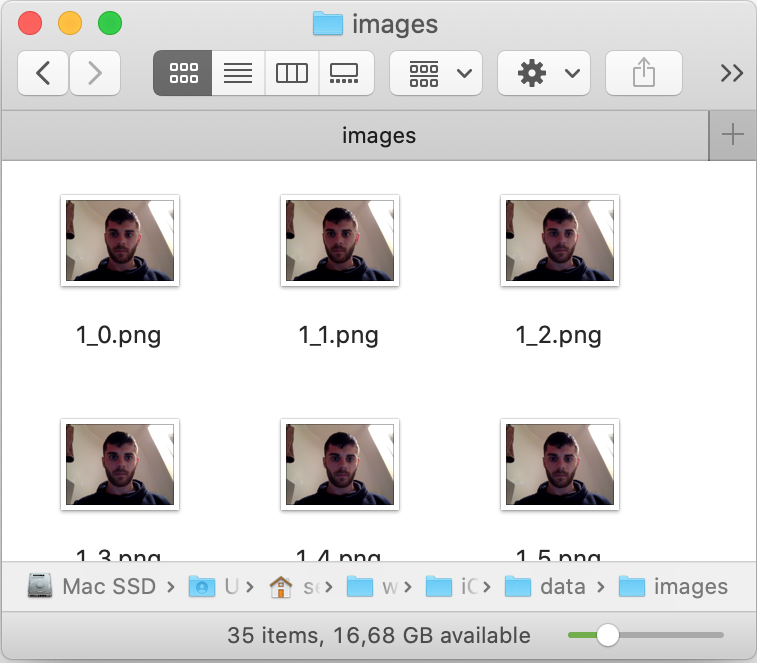
\includegraphics[width=0.7\textwidth]{data_structure_3.png}
    \caption{Cum am structurat datele}
\end{figure}

\section{Procesarea datelor}
\subsection{Avantajele unei preprocesări}
Procesarea datelor joacă un rol important în soluționarea unei probleme de învățare automată.
În primul rând, este  să eliminăm orice fel de ``zgomot'' sau informație neesențială din mulțimea noastră de date.
Apoi, putem deriva alte informații din datele inițiale, neprelucrate, informații care pot aduce un plus de performanță în soluția finală a problemei.

\subsection{Folosirea exclusivă a ochilor}
\label{data-processing:eyes}
În unele experimente, care urmează a fi prezentate în capitolul următor, m-am axat pe extragerea ochilor din imagini.
Pentru asta, am făcut uz de două biblioteci Python: dlib și imutils.
Bazându-mă pe reperele faciale care au fost prezentate în introducere\ref{figure:facial-landmarks}, am extras doar porțiunile imaginilor care delimitează ochii.

\begin{lstlisting}[language=Python, caption=Extragerea ochilor dintr-o imagine]
def extract_eyes(cv2_image):
    """Returns a list of images that contain the eyes extracted from the original image.

    First result is the left eye, second result is the right eye."""
    global _face_detector, _face_predictor
    if _detectors_are_initialised() == False:
        _initialize_detectors()

    gray_image = Utils.convert_to_gray_image(cv2_image)
    rects = _face_detector(gray_image, 0)
    if len(rects) > 0:
        shape = _face_predictor(gray_image, rects[0])
        shape = face_utils.shape_to_np(shape)

        eyes = []
        for eye in ["left_eye", "right_eye"]:
            # get the points for the contour
            (eye_start, eye_end) = face_utils.FACIAL_LANDMARKS_IDXS[eye]
            contour = shape[eye_start:eye_end]
            # get the upper left point, lower right point for this eye
            start = [min(contour, key=lambda x: x[0])[0],
                     min(contour, key=lambda x: x[1])[1]]
            end = [max(contour, key=lambda x: x[0])[0],
                   max(contour, key=lambda x: x[1])[1]]
            # extract the current eye
            eyes.append(cv2_image[start[1]:end[1], start[0]:end[0]])
        return eyes

    return None
\end{lstlisting}

Pentru prezicerea zonei în care se uită utilizatorul ne interesează mai mult contrastul dintre pupilă și iris.
Pentru aceasta, am aplicat un \emph{prag binar} (\emph{binary threshold}) imaginilor ochilor (care au fost convertite în prealabil în imagini gri) pentru a scoate în evidență poziția pupilei, relativ la întregul ochi.

\section{TODO}
TODO despre binary threshold, ce am folosit

\begin{lstlisting}[language=Python, caption=Aplicarea unui \emph{binary threshold}]
def get_binary_thresholded_image(cv2_image):
    img = convert_to_gray_image(cv2_image)
    img = cv2.medianBlur(img, 5)
    img = cv2.adaptiveThreshold(
        img, 255, cv2.ADAPTIVE_THRESH_GAUSSIAN_C, cv2.THRESH_BINARY, 11, 2)
    return img
\end{lstlisting}

\begin{figure}[h]
    \centering
    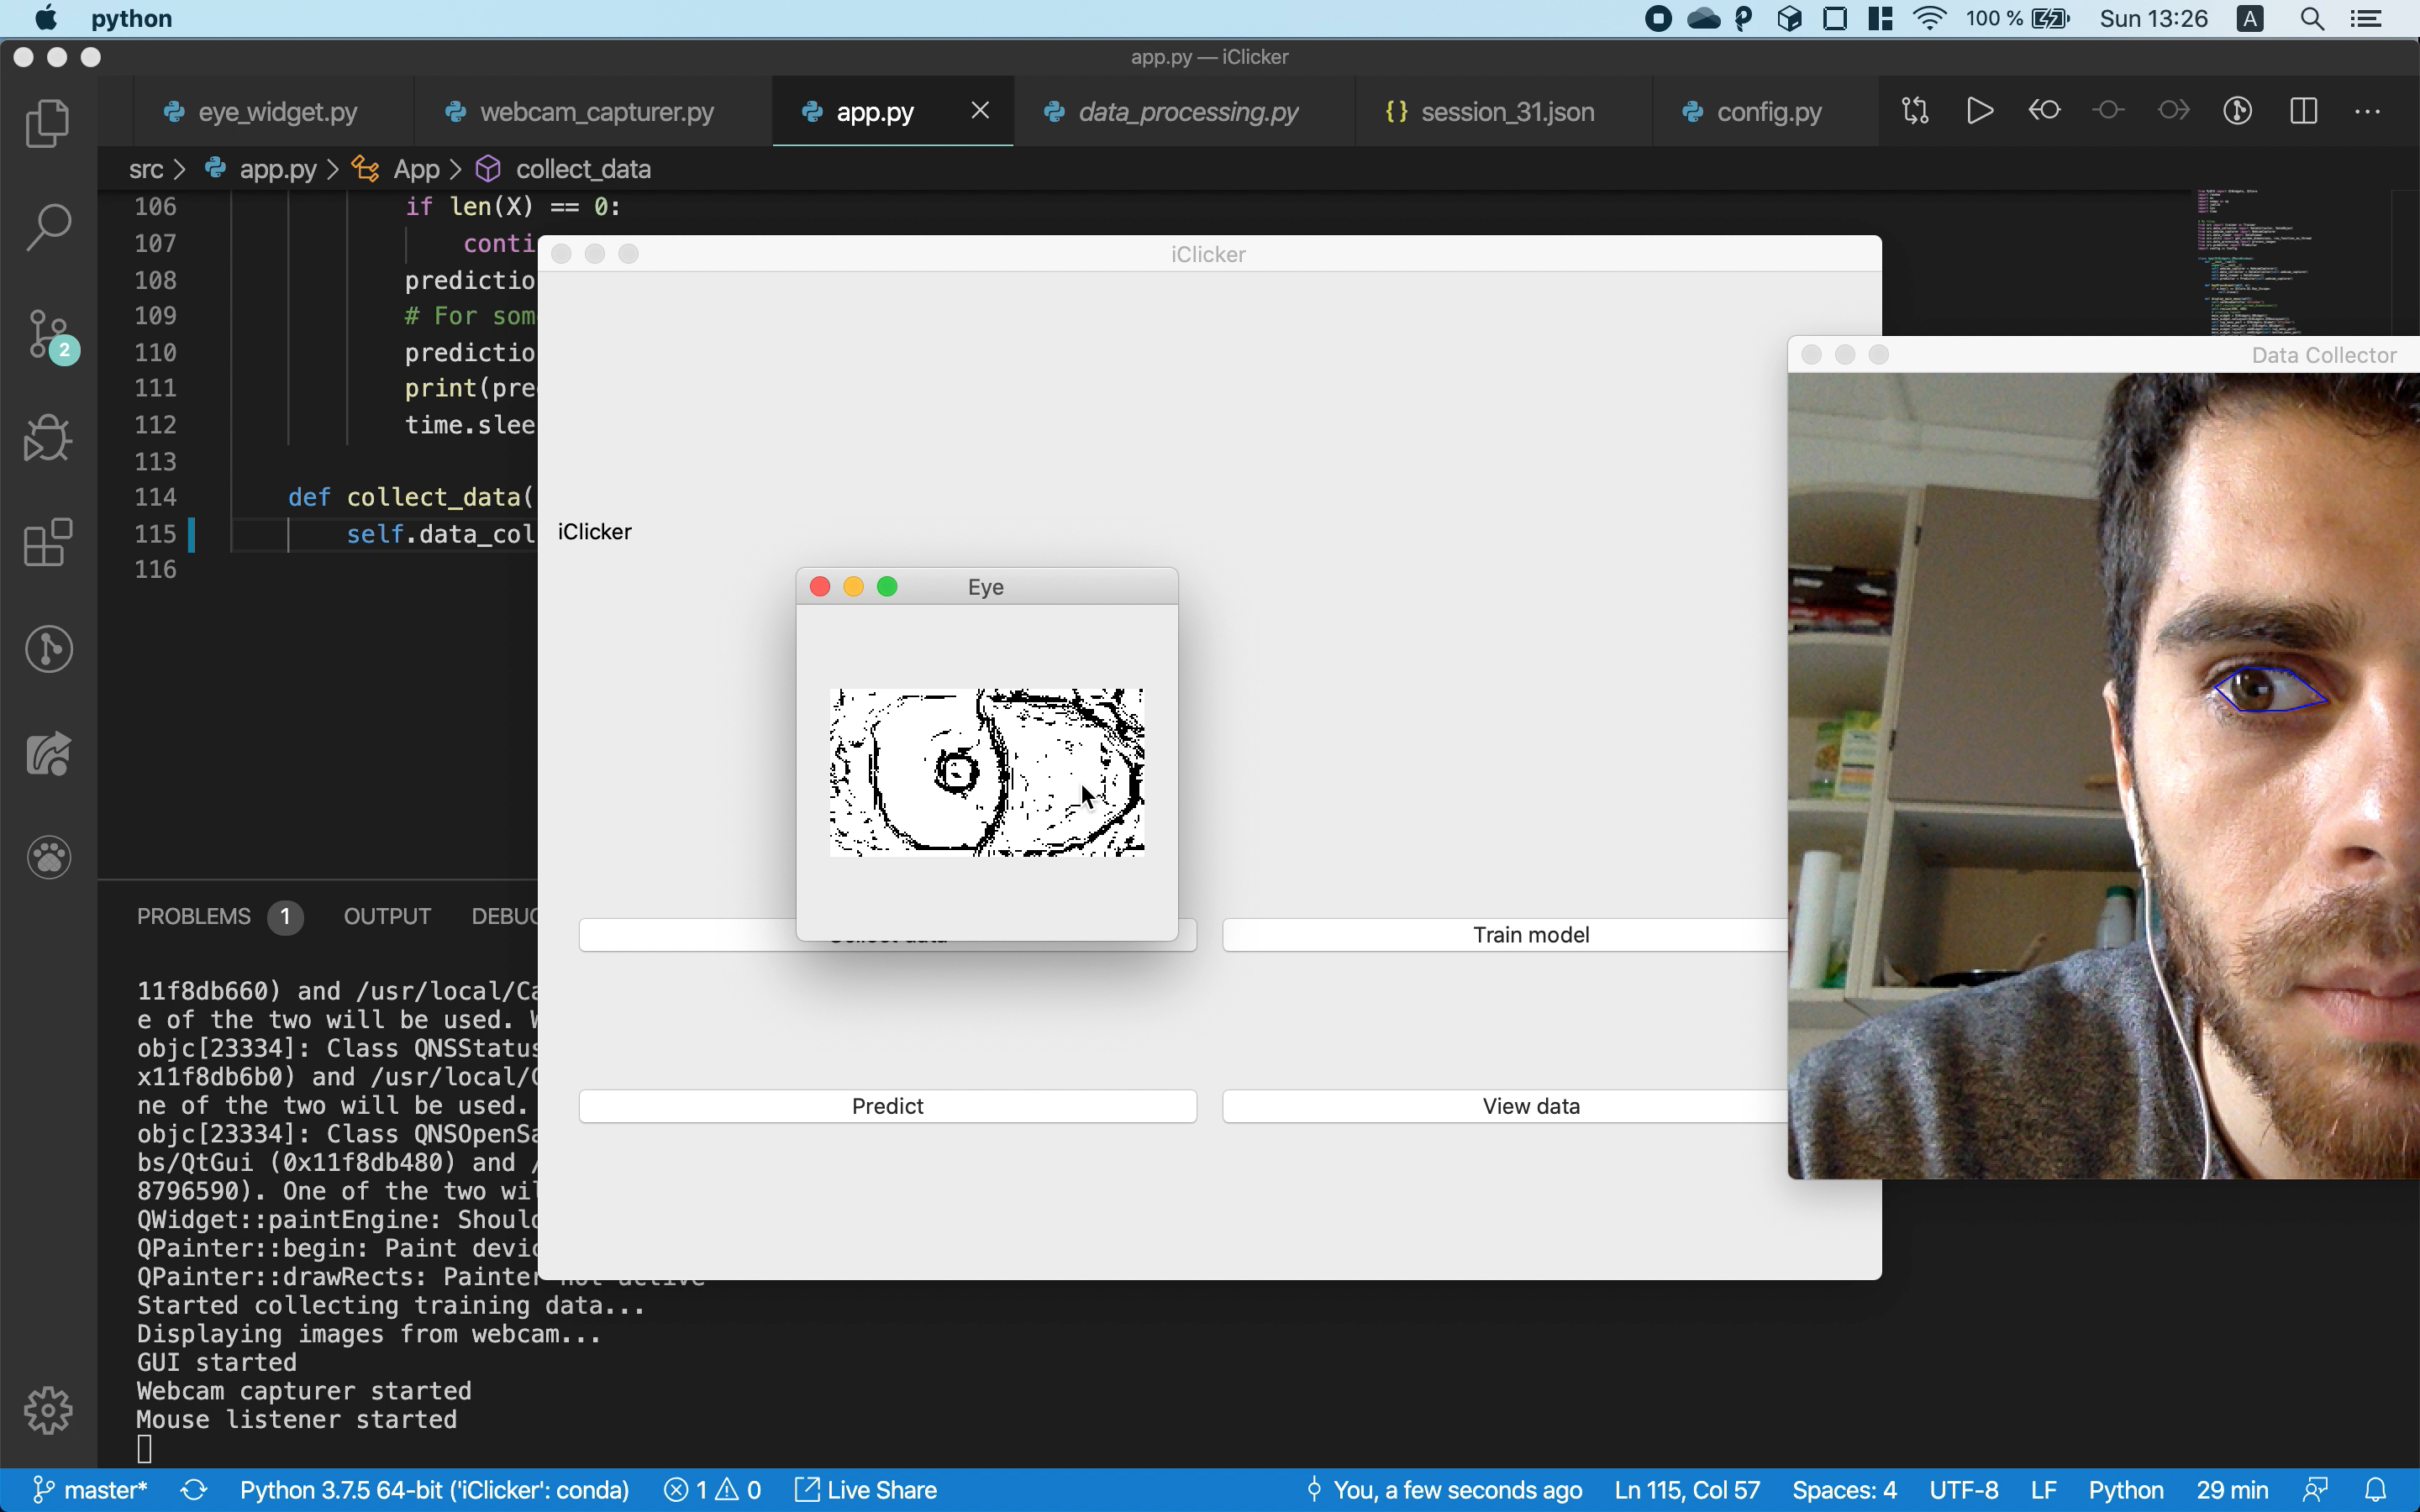
\includegraphics[width=0.49\textwidth]{eye_binary_threshold.png}
    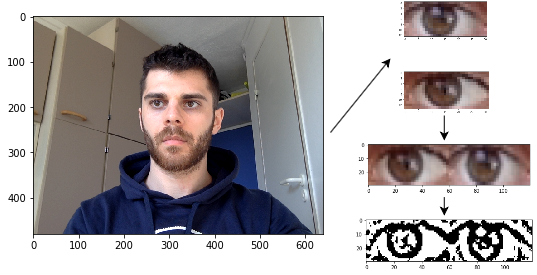
\includegraphics[width=0.49\textwidth]{threshold_process.png}
    \caption{Obținerea de informații din imaginile ochilor}
\end{figure}

\subsection{Folosirea întregii feți}
Următoarea idee a fost să folosesc fața completă a utilizatorului, apoi să o transmit unei rețele neuronale convoluționale.
Procesul de extragere a feței arată astfel:

\begin{figure}[h]
    \centering
    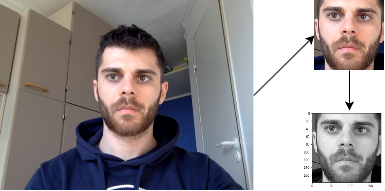
\includegraphics{extract_face_process.png}
    \caption{Extraire le visage}
    \label{fig_extracted_faces}
\end{figure}

Imaginea finală este în forma unui pătrat, conținând fața extrasă din imagine, convertită apoi in gri.
Este, de asemenea, normalizată, pentru a lua valori între $0$ și $1$.

\begin{lstlisting}[language=Python, caption=Extragerea feței dintr-o imagine]
def extract_face(cv2_image):
    """Returns the face part extracted from the image"""
    global _face_detector
    if _detectors_are_initialised() == False:
        _initialize_detectors()

    gray_image = Utils.convert_to_gray_image(cv2_image)
    rects = _face_detector(gray_image, 0)
    if len(rects) > 0:
        # only for the first face found
        (x, y, w, h) = face_utils.rect_to_bb(rects[0])
        return cv2_image[y:y+h, x:x+w]
    return None
\end{lstlisting}

\subsection{``Bandă oculară''}
Următoarea opțiune și cea care a rămas integrată în soluția finală a fost să folosesc ambii ochi, fără modificări adiționale.
Procesul de extragere a ochilor arată astfel:

\begin{figure}[h]
    \centering
    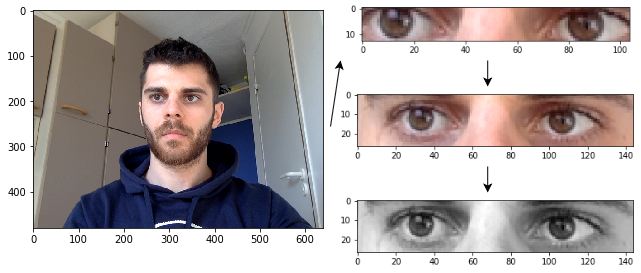
\includegraphics[width = \textwidth]{extract_eye_strip_process.png}
    \caption{Extragerea ``bandei oculare''}
    \label{fig_extracting_eye_strip}
\end{figure}

După ce am detectat fața, am extras ambii ochi, am mărit zona dreptunghiulară care încadrează ochii, pentru a avea mai multă informație, apoi am convertit imaginea în gri și am normalizat valorile pixelilor.

\begin{lstlisting}[language=Python, caption=Extragerea ``bandei oculare'' în Python3]
def extract_eye_strip(cv2_image):
    """Returns a horizontal image containing the two eyes extracted from the image"""
    global _face_detector, _face_predictor
    if _detectors_are_initialised() == False:
        _initialize_detectors()

    gray_image = Utils.convert_to_gray_image(cv2_image)
    rects = _face_detector(gray_image, 0)
    if len(rects) > 0:
        # only for the first face found
        shape = _face_predictor(gray_image, rects[0])
        shape = face_utils.shape_to_np(shape)
        (left_eye_start,
         left_eye_end) = face_utils.FACIAL_LANDMARKS_IDXS["left_eye"]
        (right_eye_start,
            right_eye_end) = face_utils.FACIAL_LANDMARKS_IDXS["right_eye"]
        # get the contour
        start, end = min(left_eye_start, right_eye_start), max(
            left_eye_end, right_eye_end)
        strip = shape[start:end]
        # get the upper left point, lower right point
        start = [min(strip, key=lambda x: x[0])[0],
                 min(strip, key=lambda x: x[1])[1]]
        end = [max(strip, key=lambda x: x[0])[0],
               max(strip, key=lambda x: x[1])[1]]
        # go a little outside the bounding box, to capture more details
        distance = (end[0] - start[0], end[1] - start[1])
        # 20 percent more details on the X axis, 60% more details on the Y axis
        percents = [20, 60]
        for i in range(0, 2):
            start[i] -= int(percents[i]/100 * distance[i])
            end[i] += int(percents[i]/100 * distance[i])
        return cv2_image[start[1]:end[1], start[0]:end[0]]
    return None

\end{lstlisting}